\documentclass{beamer}
\usetheme{Boadilla}

\usepackage[backend=biber, style=authoryear, sorting=nty]{biblatex}
\usepackage{amsmath, amssymb, amsthm, mathtools}
\usepackage{bm}
\usepackage{physics}
\usepackage{cleveref}
\usepackage{tikz}
\usepackage{pgfplots}
\pgfplotsset{compat=1.18}

\addbibresource{references.bib}

\setcounter{tocdepth}{2}


\title[Voluntary Disclosure, Personalized Pricing]{Voluntary Disclosure and Personalized Pricing}
\subtitle{Based on Ali, Lewis, and Vasserman (2022)}
\author[Theo Osterhaus]{Theo Osterhaus, 7443693}
\date[22.01.2025]{Information and Strategy, WiSe 2025/26}
\institute[WiSo]{
  Department of Economics\\
  Universität zu Köln
}



\begin{document}

\frame{\titlepage}



\begin{frame}{Outline}
    \tableofcontents
\end{frame}


\section{Introduction}
\begin{frame}{Year 2026}
    \begin{itemize}
        \setlength\itemsep{1em}
        \item \textbf{Data Availability:} Firms have ever-increasing access to consumer data, using it to target advertisements and personalise prices.
        
        \item \textbf{Regulatory Focus:} Current debates (e.g., GDPR) focus heavily on \textit{privacy} and \textit{consent}.
        
        \item \textbf{Economic Question:} Beyond privacy, we question the \textbf{distribution of surplus}. 
        \begin{itemize}
            \item Unlike early disclosure theories (Grossman, 1981; Milgrom, 1981), unravelling is not the unique outcome here.
        \end{itemize}

        \item \textbf{Research Focus:}
        We investigate what happens when consumers \textbf{fully control} their data, deciding not only \textit{whether} they are tracked, but \textit{what specific information} is disclosed.
    \end{itemize}
\end{frame}

\section{Consumer's View}
\begin{frame}{Consumer's Point of View}
    Do consumers benefit from personalised pricing when they have control over voluntarily disclosing information?

    \begin{itemize}
        \setlength\itemsep{1em}
        \item<2-> \textbf{Avoid Standard Prices (e.g., Student Discounts):}
        Sharing data allows consumers to demonstrate their eligibility for lower prices.
        
        \item<3-> \textbf{Group Leverage (e.g., Memberships):}
        Proving membership in a "price-sensitive" group forces the firm to offer a discount to secure the sale.
        
        \item<4-> \textbf{Search Efficiency (e.g., TikTok):}
        Data sharing reduces search costs. Algorithms present niche products immediately.
    \end{itemize}

    \vspace{0.4cm}

    \begin{exampleblock}{Real-World Example: Museum Ludwig (Cologne)}
        \begin{itemize}
            \item \textbf{Standard Price:} 11.00€
            \item \textbf{Discounted Price (with evidence):} 7.50€
        \end{itemize}
    \end{exampleblock}
\end{frame}

\begin{frame}{Main Research Question}
    \textbf{The Core Question:} Is there a way to weakly improve consumer surplus (CS) by disclosing evidence? Under which assumptions?

    \vspace{0.5cm}

    \begin{block}{Goal of Today}
    \begin{itemize}
        \item \textbf{Main Result:} Consumer control improves CS relative to both Perfect Price Discrimination and Uniform Pricing.
        \item \textbf{Mechanism 1 (Monopoly):} Consumers disclose \textit{partial} information (Rich Evidence) to induce group discounts.
        \item \textbf{Mechanism 2 (Competition):} Consumers use disclosure to amplify competitive forces (Simple Evidence).
    \end{itemize}
    \end{block}
\end{frame}

    \begin{frame}{Game, Notation, and Environment}
    \begin{itemize}
        \item \textbf{Players:}
        \begin{itemize}
            \item Firm $F$ (Monopolist or Competitor).
            \item Single Consumer $C$ demanding a single good.\\
        \end{itemize}
        
        \item \textbf{Valuation ($v$):}
        \begin{itemize}
            \item $v \in [a,b]$ represents the valuation of $C$ for good.
            \item Based on observable data (e.g., buying habits, location, gender).
        \end{itemize}
        
        \item \textbf{Evidence Strategy:}
        \begin{itemize}
            \item Consumer chooses a message $m$ from a set $\mathcal{M}(v)$.
            \item The message contains proof that $v \in m$ (Hard Information).
        \end{itemize}
    \end{itemize}

    \begin{block}{Assumptions \& Solution Concept}
        We study the PBE \textbf{Perfect Bayesian Equilibrium (A\ref{PBE})}.
        \begin{itemize}
            \item \textbf{Rationality:} $F$ and $C$ behave sequentially rationally.
            \item Consistent beliefs (Bayes' Rule).
            \item \textbf{Tie-Breaking:} If indifferent, $C$ chooses to buy the good.
        \end{itemize}
    \end{block}
\end{frame}

\section{Monopoly Market}
\subsection{Benchmark Solution}
\begin{frame}{Benchmark: Standard Monopoly (No Disclosure)}
    \begin{itemize}
        \item \textbf{Setup:}
        \begin{itemize}
            \item Monopolist $M$, Marginal Cost $c=2$.
            \item Consumer $v \sim \mathcal{U}[1,10]$.
        \end{itemize}
    \end{itemize}

    \textbf{Problem:} $M$ maximizes expected profit without disclosure:
    \begin{align*}
        \max_{p} \pi(p) &= (p - c) \times \mathbb{P}(v \ge p) \\
        &= (p - 2) \left( \frac{10 - p}{9} \right)
    \end{align*}

    \textbf{Solution:}
    \begin{itemize}
        \item FOC: $12 - 2p = 0 \implies \mathbf{p^* = 6}$
        \item Profit: $\mathbf{\pi \approx 1.78}$
        \item Consumer Surplus: $\mathbf{CS \approx 0.89}$
    \end{itemize}
    \footnotesize{\textit{(Detailed derivation in Appendix: P\ref{MB})}}
\end{frame}

\subsection{Simple Evidence}
\begin{frame}{Simple Evidence: The Unravelling Result}
    \textbf{Definition:} $\mathcal{M}(v) = \{ \{v\}, \emptyset \}$. The consumer can only Reveal All ($m=v$) or Stay Silent ($m=\emptyset$). ("All-or-Nothing")

    \vspace{0.3cm}

    \begin{enumerate}
        \item \textbf{Strategy: Full Revelation ($m=v$)}
        \begin{itemize}
            \item If the consumer reveals that the monopolist sets $p=v$.
            \item \textbf{Result:} $CS=0$ and $PR = 3.56$ (Perfect Price Discrimination).
        \end{itemize}
        
        \vspace{0.2cm}
        \item \textbf{The "Punishing Belief" (Silence)}
        \begin{itemize}
            \item If the consumer is silent (Non-Disclosure), the monopolist infers they must be a high-value type trying to hide.
            \item \textit{Logic:} "Only a consumer with the highest valuation would refuse to prove otherwise."
            \item \textbf{Equilibrium:} The price for non-disclosure rises to $p_{ND} = 10$.
        \end{itemize}
    \end{enumerate}

    \begin{alertblock}{Result}
        Simple evidence leads to \textbf{Full Revelation} as \textbf{PBE}. Consumers are forced to disclose to avoid the high punishment price, and the Monopolist captures all surplus.
    \end{alertblock}
\end{frame}


    \begin{frame}{Conclusion: The Limits of Simple Evidence}
        \begin{itemize}
            \setlength\itemsep{1em}
            \item \textbf{Welfare Impact:} 
            \begin{itemize}
                \item Simple evidence generally cannot improve consumer welfare; it often hurts it.
                \item Full revelation allows the monopolist to achieve Perfect Price Discrimination, capturing all surplus.
            \end{itemize}
            
            \item \textbf{Forced Revelation:}
            \begin{itemize}
                \item A monopolist can use "sceptical beliefs" to force consumers to reveal their data.
                \item Even if a consumer wants to hide, the high default price ($p_{ND}=10$) compels them to disclose to get a slightly better price, leading to total unravelling.
            \end{itemize}
        \end{itemize}
    
        \begin{block}{Proposition 1}
            With simple evidence, across all equilibria, the consumer's interim payoff is bounded above, no more than her payoff from uniform pricing by $\max\{v - p^*, 0\}$.\cite{10.1093/restud/rdac033}
        \end{block}
    
        \vspace{0.2cm}
        \footnotesize{\textit{Note: Similar results hold for discrete distributions (e.g., $v \in \{1, 10\}$).} P\ref{Mdiscrete}}
    \end{frame}


\subsection{Rich Evidence}
\begin{frame}{Rich Evidence}
        \begin{itemize}
            \setlength\itemsep{1em}
            \item \textbf{The Opportunity:}
            Assume Monopolist $M$ can offer group discounts for different consumer segments.
             \item \textbf{The Dilemma:}
            \begin{itemize}
                \item If $C$ fully reveals their exact valuation ($m=v$), the Monopolist extracts all surplus ($CS=0$).
                \item If $C$ stays silent, the Monopolist assumes the worst (highest type) and charges a massive price ($p_{ND}=10$).
            \end{itemize}
            \item \textbf{Consumer Incentive:}
            Consumer $C$ has an incentive to verify that their valuation belongs to a lower-value segment to gain a discount. $C$ is able to send $m=[a,b]: v \in m$
            \item \textbf{The Question:}
            Is there a way for the consumer to prove they are a "low type" ($C_l$) without revealing their \textit{exact} valuation?
        \end{itemize}
    \end{frame}
    
\begin{frame}{Zeno's Partition: The Mechanism}
        \begin{itemize}
            \item There exists an equilibrium where groups of customers benefit from disclosing partial information to access group discounts.
            \item Consumers pool into "buckets" to hide their exact value while still proving they are not high-value types.
            \item \textbf{Zeno's Partition:} The interval is divided into segments ($S_1, S_2, S_3, \dots$) where each segment is half the size of the one above it (e.g., $S_1$ is width 4, $S_2$ is width 2).
        \end{itemize}
    
        \begin{figure}
            \centering
            
\includegraphics[width=0.6\linewidth]{MarginalCosts.png}
            \caption{Partition Structure accumulating at Marginal Cost $c=2$}
            \label{fig:zeno_structure}
        \end{figure}        
 \end{frame}

\begin{frame}{Equilibrium Prices and Consumer Surplus}
        With rich evidence, the consumer's disclosure strategy generates the following stepped price function:
    
        \begin{figure}
            \centering
            % Ensure this image file exists in your directory
            \includegraphics[width=0.75\linewidth]{eqpricesandcs.png}
            \caption{Equilibrium Prices and Consumer Surplus ($c=2$)}
            \label{fig:eq_prices}
        \end{figure}
        
    \end{frame}
\begin{frame}{Calculating Welfare Gains}
        \textbf{1. Total Producer Revenue Normalised (PR):}
        Using the geometric series sum formula where $a = PR_{S1} = 16$ and $r = 1/4$:
        \begin{align*}
            \text{PR} &= \frac{1}{9} \times \frac{a}{1-r} = \frac{1}{9} \times \frac{16}{1 - 0.25} \\
                      &= \frac{1}{9} \times 21.33 = \mathbf{2.37}
        \end{align*}
    
        \textbf{2. Total Consumer Surplus Normalised (CS):}
        Using $a = CS_{S1} = 8$ and $r = 1/4$:
        \begin{align*}
            \text{CS} &= \frac{1}{9} \times \frac{a}{1-r} = \frac{1}{9} \times \frac{8}{1 - 0.25} \\
                      &= \frac{1}{9} \times 10.67 = \mathbf{1.19}
        \end{align*}
    \end{frame}
    
    \begin{frame}{Welfare Implications}
        \begin{itemize}
            \item \textbf{Consumer Surplus Result:} 
            CS increases for almost all types compared to the benchmark. Consumers effectively force the monopolist to lower prices.
            
            \item \textbf{Pareto Improvement:} 
            Interestingly, this leads to a Pareto improvement:
            \begin{itemize}
                \item \textbf{Efficient Trade:} Total social value is maximised (no Deadweight Loss).
                \item \textbf{Win-Win:} Neither party is worse off than in the standard monopoly baseline.
            \end{itemize}
            \item \textbf{Real-World Parallel:} This theoretical result mirrors "Group Discounts" seen in practice (e.g., Student or Senior discounts).
        \end{itemize}
        
        \vspace{0.2cm}
        
        \begin{block}{Takeaway}
            There are worse equilibria for CS, but no equilibrium achieves higher \textit{ex ante} CS than Zeno's Partition.
        \end{block}
    \end{frame}
    
    \begin{frame}{Comparison}
    \begin{table}[h!]
        \centering
        % \resizebox ensures the table fits the width of the slide frame
        \resizebox{\textwidth}{!}{%
        \renewcommand{\arraystretch}{1.3} % Adds slight vertical breathing room
        \begin{tabular}{lccc}
            \hline
            Metric & Benchmark & Simple Evidence & Rich Evidence \\
             & (Standard Monopoly) & (Full Disclosure) & (Zeno's Partition) \\
            \hline
            \hline
            Pricing Strategy & Single Price ($p=6$) & Personalized ($p=v$) & Step Function ($p \in \{6, 4, \dots\}$) \\
            \hline
            Producer Revenue (PR) & 1.78 & 3.56 & 2.37 \\
            \hline
            Consumer Surplus (CS) & 0.89 & 0.00 & 1.19 \\
            \hline
            Total Welfare & 2.67 & 3.56 & 3.56 \\
            \hline
            Efficiency & Inefficient & Efficient & Efficient \\
            \hline
        \end{tabular}%
        }
        \caption{Comparison of Equilibrium Outcomes ($c=2, v \in [1,10]$)}
    \end{table}
        \end{frame}
          
\section{Bertrand Competition}

\begin{frame}{Game: Bertrand with Horizontal Differentiation}
    \begin{itemize}
        \item \textbf{Setup: The "Smartphone Switcher" Paradox}
        \begin{itemize}
            \item Firms are at opposite ends of the Hotelling line:\\
                \textbf{Apple ($A$)} at $l_a = -1000$ \quad vs. \quad \textbf{Samsung ($S$)} at $l_s = 1000$
            \item Consumer $C$ location $l_c \sim \mathcal{U}[-1000, 1000]$.
        \end{itemize}
    \end{itemize}

    \vspace{0.3cm}
    
    \textbf{Problem:} Without disclosure, Firm $A$ maximizes expected profit.
    
    \vspace{0.2cm}

    \textbf{Benchmark Solution:}
    \begin{itemize}
        \item Solving the FOC yields the standard "Hotelling" price:
        \[ p^* = \mathbf{2000} \quad \text{and} \quad \pi^* = \mathbf{1000} \]
     \end{itemize}
     \vspace{0.2cm}
     \footnotesize{\textit{(Detailed derivation in Appendix: P\ref{BB})}}
\end{frame}


\begin{frame}{Equilibrium Disclosure Strategies} 
    \textbf{PBE with Simple Evidence}
    \begin{itemize}
        \item Consumers privately send messages: $m=v$ (exact location) or $m=[-1000,1000]$ (silence).
        \item This creates two independent tracking decisions (one for each firm).
    \end{itemize}

    \vspace{0.5cm}
    
    \centering
    \textbf{PBE: Disclosure Strategy by Consumer Location}
    
    \vspace{0.3cm}

        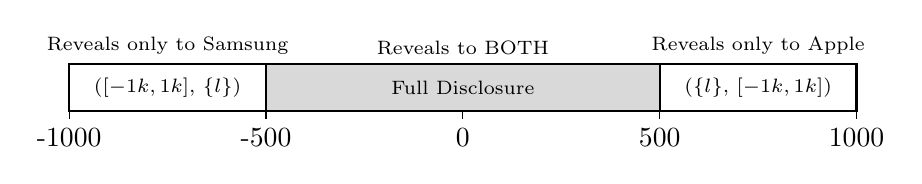
\begin{tikzpicture}[xscale=5]
            % Draw the main horizontal line
            \draw[thick] (-1, 0) -- (1, 0);
            
            % Draw tick marks and labels (RESCALED TO MATCH -1000 to 1000)
            \draw (-1, 0.1) -- (-1, -0.1) node[below] {-1000};
            \draw (-0.5, 0.1) -- (-0.5, -0.1) node[below] {-500};
            \draw (0, 0.1) -- (0, -0.1) node[below] {0};
            \draw (0.5, 0.1) -- (0.5, -0.1) node[below] {500};
            \draw (1, 0.1) -- (1, -0.1) node[below] {1000};
            
            % Segment 1: Reveals to Samsung (Far)
            \draw[thick] (-1, 0) rectangle (-0.5, 0.6);
            \node[above, font=\scriptsize] at (-0.75, 0.6) {Reveals only to Samsung};
            \node[font=\scriptsize] at (-0.75, 0.3) {($[-1k, 1k]$, $\{l\}$)};
            
            % Segment 2: Reveals to Both (Middle)
            \draw[thick, fill=gray!30] (-0.5, 0) rectangle (0.5, 0.6);
            \node[above, font=\scriptsize] at (0, 0.6) {Reveals to BOTH};
            \node[font=\scriptsize] at (0, 0.3) {Full Disclosure};
            
            % Segment 3: Reveals to Apple (Far)
            \draw[thick] (0.5, 0) rectangle (1, 0.6);
            \node[above, font=\scriptsize] at (0.75, 0.6) {Reveals only to Apple};
            \node[font=\scriptsize] at (0.75, 0.3) {($\{l\}$, $[-1k, 1k]$)};
        \end{tikzpicture}
    
    \vspace{0.2cm}
    {\footnotesize \textit{Extreme types reveal only to the rival. Centre types reveal to everyone.}}
\end{frame}


\begin{frame}{The Mechanism: Why Reveal to the Rival?}
    Consider a consumer at $l \in [500, 1000]$ (A "Samsung Loyalist").

    \begin{columns}[T]
        \begin{column}{0.48\textwidth}
            \textbf{1. The Threat (Apple)}
            \begin{itemize}
                \item Consumer reveals location to Apple.
                \item Apple knows it has a disadvantage.
                \item Apple bids \textbf{Marginal Cost ($p_A=0$)} to poach.
            \end{itemize}
        \end{column}
        \begin{column}{0.48\textwidth}
            \textbf{2. The Protection (Samsung)}
            \begin{itemize}
                \item Consumer stays \textbf{silent} with Samsung.
                \item Samsung must match Apple's offer to keep the customer.
                \item Result: Samsung lowers to a limit price of $p_S = 1000$.
            \end{itemize}
        \end{column}
    \end{columns}

    \vspace{0.3cm}
    \begin{block}{Welfare Gain}
        \[
            \underbrace{1000 + (1000 - l)}_{\text{Total Exp. (Disclosure)}} \quad \le \quad \underbrace{2000 + (1000 - l)}_{\text{Total Exp. (Benchmark)}}
        \]
        \textit{The consumer pays strictly less than without disclosure.}
    \end{block}
    \footnotesize{\textit{(Detailed derivation in Appendix: P\ref{Bertrand})}}
\end{frame}

\section{Discussion \& Conclusion}
\begin{frame}{Discussion}
    \begin{itemize}
        \setlength\itemsep{1em}
        \item \textbf{The Core Question:} Can consumers benefit from sharing their private information?
        \item \textbf{Welfare Gains:} Giving consumers control over their data can generate substantial gains to welfare, provided the right technologies exist. Which depend on market structure and disclosure technology.
        \item \textbf{Key Mechanism:} The ability to \textbf{selectively disclose} information is central to realizing these gains.
    \end{itemize}

    \begin{alertblock}{Policy Implication}
        Without regulation ensuring \textbf{consumer control} (selective disclosure), firms may design systems that prevent selective disclosure, that erase these welfare gains predicted by the model.
    \end{alertblock}
\end{frame}



\begin{frame}{Practical Obstacles}
    \begin{itemize}
         \item \textbf{The Paradox of Preference Intensity:}
        \begin{itemize}
            \item \textbf{Monopoly:} Revealing high intensity ($v$) leads to \textbf{exploitation}.
            \item \textbf{Competition:} Revealing high intensity ($l$) leads to \textbf{aggressive poaching} (discounts).
            \item The Paradox: The same data point ('I love this product') has the opposite effect depending on market structure."
        \end{itemize}
        
        \item \textbf{Data Leakage:} If data leaks (e.g., via brokers), it undermines the consumer's ability to \textit{selectively} disclose.

        \item \textbf{Data Brokers:} Third-party brokers acquire data, complicating the distribution of welfare.
    \end{itemize}
\end{frame}

\section*{Bibliography}
\begin{frame}{Bibliography}
    \printbibliography
\end{frame}
    
\appendix
\section*{Appendix}

\begin{frame}{Formal Definition: PBE} \label{PBE}
    \textbf{Perfect Bayesian Equilibrium (PBE)} requires:
    \vspace{0.2cm}
    \begin{enumerate}
        \item \textbf{Sequential Rationality:} 
        At every information set, players choose strategies that maximise their expected payoffs, given their beliefs and the strategies of others.
        
        \item \textbf{Consistency of Beliefs:} 
        Beliefs ($\mu$) are derived from equilibrium strategies using Bayes' Rule wherever possible.
    \end{enumerate}

    \vspace{0.4cm}
    \textbf{Application to Our Model:}
    \begin{itemize}
        \item \textbf{Consumer Strategy:} Choose message $m \in \mathcal{M}(v)$ to minimize the final purchase price.
        \item \textbf{Firm Beliefs:} Upon receiving $m$, update belief about $v$. If $m$ is off-path (e.g., silence when disclosure is expected), form "sceptical beliefs."
        \item \textbf{Firm Strategy:} Set price $p(m)$ to maximize profit given updated beliefs.
    \end{itemize}
\end{frame}

\begin{frame}{Derivation: Monopoly Benchmark}\label{MB}
    \textbf{Problem:} Without disclosure, Monopolist $M$ maximizes expected profit.
    
    \begin{itemize}
        \item \textbf{Demand:} $v \sim \mathcal{U}[1,10]$. Probability of sale at price $p$:
        \[ \mathbb{P}(v \ge p) = \frac{10 - p}{9} \]
        \item \textbf{Profit Function:}
        \[ \pi(p) = (p - c) \cdot \mathbb{P}(v \ge p) = (p - 2) \left( \frac{10 - p}{9} \right) \]
    \end{itemize}

    \textbf{Optimisation (FOC):}
    \begin{align*}
        \frac{d\pi}{dp} = \frac{1}{9} \left[ (10-p) + (p-2)(-1) \right] &= 0 \\
        10 - p - p + 2 &= 0 \\
        12 - 2p &= 0 \implies \mathbf{p^* = 6}
    \end{align*}
    
    \textbf{Welfare:}
    \[ \pi^* = (6-2)\frac{4}{9} \approx 1.78, \quad CS = \frac{1}{2}(4)(\frac{4}{9}) \approx 0.89 \]
\end{frame}

\begin{frame}{Monopoly Benchmark: Consumer Surplus (CS)}
    \begin{itemize}
        \item \textbf{Consumer Surplus (CS):}
        Calculated as the accumulated surplus for all consumers with $v \ge p^*$:
        \[
            CS = \int_{p^*}^{10} (v - p^*) f(v) \, dv = \int_{6}^{10} (v - 6) \frac{1}{9} \, dv
        \]
        \[
            = \frac{1}{9} \left[ \frac{(v-6)^2}{2} \right]_{6}^{10} = \frac{1}{9} \left( \frac{16}{2} - 0 \right) = \frac{8}{9} \approx \mathbf{0.89}
        \]
    \end{itemize}
\end{frame}

\begin{frame}{Monopoly: Discrete Example}\label{Mdiscrete}
    \begin{itemize}
        \item \textbf{Setup:}
        \begin{itemize}
            \item Monopolist $M$ produces good $G$ with marginal cost $c=5$.
            \item Consumer $C$ has discrete valuation $v \in \{20, 30\}$ with equal probability:
            \[
                \mathbb{P}(v=20) = \mathbb{P}(v=30) = \frac{1}{2}
            \]
        \end{itemize}
    \end{itemize}

    \vspace{0.3cm}

    \textbf{Benchmark Problem:} Without disclosure, Monopolist maximizes expected profit:
    \begin{align*}
        \max_{p} \pi(p) &= (p - c) \times \mathbb{P}(v \ge p)
    \end{align*}

    \textbf{Strategies:}
    The monopolist considers the feasible price points:
    \begin{enumerate}
        \item \textbf{Low Price ($p=20$):} Sells to both types ($\mathbb{P} = 1$).
        \item \textbf{High Price ($p=30$):} Sells only to high types ($\mathbb{P} = 0.5$).
        \item \textbf{Prohibitive Price ($p > 30$):} Sells to no one ($\mathbb{P} = 0$).
    \end{enumerate}
\end{frame}

\begin{frame}{Monopoly: Discrete Example}
    \textbf{1. Compare Profits:}
    \begin{itemize}
        \item \textbf{Case A ($p=20$):}
        \[
            \pi(20) = (20 - 5) \times 1 = \mathbf{15}
        \]
        \item \textbf{Case B ($p=30$):}
        \[
            \pi(30) = (30 - 5) \times 0.5 = 25 \times 0.5 = \mathbf{12.5}
        \]
    \end{itemize}
    
    \vspace{0.2cm}
    \textbf{Result:} The monopolist chooses optimal price $\boxed{p^* = 20}$.

    \vspace{0.4cm}
    \textbf{2. Welfare Analysis (Consumer Surplus):}
    \begin{itemize}
        \item \textbf{Low Type ($v=20$):} $CS_L = 20 - 20 = 0$.
        \item \textbf{High Type ($v=30$):} $CS_H = 30 - 20 = 10$.
        \item \textbf{Expected CS:}
        \[
            \mathbb{E}[CS] = 0.5(0) + 0.5(10) = \mathbf{5}
        \]
    \end{itemize}
\end{frame}

\begin{frame}{Monopoly: Discrete Example}
    \begin{itemize}
        \item \textbf{Strategy 1: Full Disclosure ($m=v$)}
        \begin{itemize}
            \item Low type ($v=20$) reveals $\rightarrow$ Firm charges $p=20$. ($CS=0$).
            \item High type ($v=30$) reveals $\rightarrow$ Firm charges $p=30$. ($CS=0$).
            \item \textit{Result:} Monopolist extracts all surplus.
        \end{itemize}
        
        \vspace{0.4cm}

        \item \textbf{Strategy 2: Non-Disclosure (Silence)}
        \begin{itemize}
            \item \textbf{Punishing Belief:} If the consumer says nothing, the monopolist infers they must be the \textbf{high type} ($v=30$) trying to hide.
            \item The firm sets $p=30$.
            \item \textbf{Outcome:} The high type pays 30 anyway; the low type is priced out of the market.
        \end{itemize}
    \end{itemize}

    \vspace{0.2cm}
    \begin{block}{Conclusion}
        Just like in the continuous case, Simple Evidence leads to unraveling ($CS \to 0$).
    \end{block}
\end{frame}

\begin{frame}{Bertrand: Standard Hotelling model}\label{BB}
    We consider a standard Hotelling model with two firms located at opposite ends of a line segment and a single consumer with unknown location.

\begin{itemize}
    \item \textbf{Firms:} Apple ($A$) is located at $l_A = -1000$ and Samsung ($S$) is located at $l_S = 1000$.
    \item \textbf{Consumer:} The consumer's location $x$ is uniformly distributed on the interval $[-1000, 1000]$, i.e., $x \sim \mathcal{U}[-1000, 1000]$.
    \item \textbf{Transport Cost:} Linear transport costs are assumed (distance from the firm).
\end{itemize}

A consumer at location $\hat{x}$ is indifferent between purchasing from Apple or Samsung if the total cost (Price + Transport Cost) is equal for both options:
\begin{equation}
    p_A + |\hat{x} - (-1000)| = p_S + |1000 - \hat{x}|
\end{equation}
\end{frame}

\begin{frame}{Bertrand: Standard Hotelling model}
Assuming the indifferent consumer lies between the firms, this simplifies to:
\begin{align}
    p_A + (\hat{x} + 1000) &= p_S + (1000 - \hat{x}) \\
    2\hat{x} &= p_S - p_A \\
    \hat{x} &= \frac{p_S - p_A}{2}
\end{align}
Apple captures all consumers to the left of $\hat{x}$ (i.e., $x < \hat{x}$).

Since the consumer's location is uniformly distributed over a total length of $2000$ (from $-1000$ to $1000$), the probability that Apple wins the customer is the portion of the line to the left of $\hat{x}$:
\begin{equation}
    \mathbb{P}(\text{A wins}) = \frac{\hat{x} - (-1000)}{2000} = \frac{\frac{p_S - p_A}{2} + 1000}{2000}
\end{equation}
Simplifying the fraction:
\begin{equation}
    \mathbb{P}(\text{A wins}) = \frac{p_S - p_A + 2000}{4000}
\end{equation}    
\end{frame}

\begin{frame}{Bertrand: Standard Hotelling model}
    Apple chooses price $p_A$ to maximize its expected profit, given Samsung's price $p_S$[cite: 454]:
\begin{equation}
    \max_{p_A} \mathbb{E}[\pi_A] = p_A \times \mathbb{P}(\text{A wins}) = p_A \left( \frac{p_S - p_A + 2000}{4000} \right)
\end{equation}
To find the optimal price, we take the First Order Condition (FOC) with respect to $p_A$:
\begin{align}
    \frac{\partial \mathbb{E}[\pi_A]}{\partial p_A} &= \frac{1}{4000} \left[ (p_S - p_A + 2000) + p_A(-1) \right] = 0 \\
    p_S - 2p_A + 2000 &= 0
\end{align}

Assuming a symmetric equilibrium where $p_A = p_S = p^*$:
\begin{align}
    p^* - 2p^* + 2000 &= 0 \\
    -p^* &= -2000 \\
    p^* &= 2000
\end{align}
\end{frame}

\begin{frame}{Bertrand: Standard Hotelling model}
The expected profit for each firm is then:
\begin{equation}
    \pi^* = p^* \times \frac{1}{2} = 2000 \times 0.5 = 1000
\end{equation}
This confirms that uncertainty about the consumer's location allows firms to maintain high prices ($p^* > MC$), as opposed to the Bertrand paradox outcome where $p=MC$.
\end{frame}

\begin{frame}{Equilibrium Logic: The "Samsung Loyalist" ($l \in [500, 1000]$)}\label{Bertrand}
    Consider a consumer located in the interval $[500, 1000]$. They are physically closer to Samsung ($1000$) than Apple ($-1000$).

    \vspace{0.2cm}

    \textbf{Step 1: Disclosure to Rival (The Threat)}
    \begin{itemize}
        \item The consumer reveals their location to \textbf{Apple}.
        \item Apple sees it is at a massive disadvantage (distance $>1500$).
        \item \textbf{Reaction:} To compete, Apple drops its price to Marginal Cost: $\mathbf{p_A = 0}$.
        \item \textit{Outcome:} The consumer secures an outside option with total cost:
        \[ \text{Cost}_A = p_A + |l - (-1000)| = 0 + (l + 1000) \approx 1500 \text{ (at cutoff)} \]
    \end{itemize}

\end{frame}

\begin{frame}{Equilibrium Logic: The "Samsung Loyalist" ($l \in [500, 1000]$)}
     \textbf{Step 2: Silence to Preferred Firm (The Protection)}
    \begin{itemize}
        \item The consumer stays silent with \textbf{Samsung}.
        \item Samsung infers the consumer is in $[500, 1000]$ but cannot price discriminate individually. It sets a single \textbf{Limit Price ($p_S$)}.
    \end{itemize}

    \textbf{Step 3: Finding the Equilibrium Price ($p_S$)}
    Samsung must price low enough to retain the "most tempted" customer (at $l=500$):
    \begin{align*}
        \text{Cost}_S(500) &\le \text{Cost}_A(500) \\
        p_S + |1000 - 500| &\le 0 + |500 - (-1000)| \\
        p_S + 500 &\le 1500 \\
        \mathbf{p_S} &= \mathbf{1000}
    \end{align*}

    \begin{block}{Result}
        By revealing only to the rival, the consumer forces Samsung to charge $\mathbf{p_S = 1000}$ (half the benchmark price), resulting in total expenditure $\mathbf{2000 - l}$.
    \end{block}
\end{frame}


\end{document}